\documentclass[12pt,a4paper]{article}

\usepackage{fontspec}
\usepackage{polyglossia}
\setmainlanguage{polish}
\usepackage{amsmath}
\usepackage{amssymb}
\usepackage{booktabs}
\usepackage{caption}
\usepackage{float}
\usepackage{geometry}
\usepackage{graphicx}
\usepackage{hyperref}

\geometry{margin=2.5cm}
\graphicspath{{assets/}}
\hypersetup{
    colorlinks=true,
    linkcolor=black,
    citecolor=black,
    urlcolor=blue
}

\title{Kompresja danych EKG z użyciem sztucznej sieci neuronowej typu MLP}
\author{Kacper Wojtowicz \and Gracjan Adamus \and Dominik Godek \and Rafał Wybraniec}
\date{\today}

\begin{document}
\maketitle

\begin{abstract}
W sprawozdaniu opisano projekt kompresji jednowymiarowych przebiegów EKG z użyciem autoenkodera opartego na wielowarstwowym perceptronie. Zadanie polegało na nauczeniu sieci neuronowej, która odwzorowuje wektor 187 próbek pojedynczego uderzenia serca do krótszej reprezentacji latentnej, a następnie rekonstruuje przebieg wejściowy. Do eksperymentów wykorzystano zbiór \textit{ECG Heartbeat Categorization Dataset} z portalu Kaggle, przygotowany na podstawie baz MIT-BIH Arrhythmia Database i PTB Diagnostic ECG Database. Zbadano kilka wymiarów warstwy wąskiego gardła i wyznaczono zależność pomiędzy stopniem kompresji a jakością odtworzenia sygnału. Wyniki autoenkodera MLP porównano z metodą PCA, traktowaną jako liniowy punkt odniesienia.
\end{abstract}

\tableofcontents
\newpage

\section{Cel i zakres projektu}
Celem projektu było opracowanie i przetestowanie koncepcji kompresji przebiegów EKG przy użyciu sztucznej sieci neuronowej. Rozważany system miał działać dwukierunkowo:
\begin{itemize}
    \item jako kompresor, czyli enkoder przekształcający sygnał EKG do krótszego wektora cech,
    \item jako dekompresor, czyli dekoder rekonstruujący sygnał z reprezentacji skompresowanej.
\end{itemize}

Przyjęto, że pojedynczy rekord danych jest wektorem:
\[
    \mathbf{x} = [x_1, x_2, \ldots, x_{187}] \in [0,1]^{187}.
\]
Autoenkoder generuje reprezentację latentną:
\[
    \mathbf{z} = f_\theta(\mathbf{x}) \in \mathbb{R}^{K},
\]
gdzie $K$ oznacza wymiar wąskiego gardła. Dekoder odtwarza sygnał:
\[
    \hat{\mathbf{x}} = g_\phi(\mathbf{z}).
\]
Wartość $K$ decyduje o sile kompresji. Im mniejsze $K$, tym większy stopień kompresji, ale zwykle także większy błąd rekonstrukcji.

\section{Dane wejściowe}
\subsection{Opis zbioru}
Źródłem danych był zbiór Kaggle \textit{ECG Heartbeat Categorization Dataset} \cite{kaggleheartbeat}. Zbiór ten zawiera przetworzone sygnały uderzeń serca pochodzące z publicznych baz MIT-BIH Arrhythmia Database oraz PTB Diagnostic ECG Database. Artykuł Kachuee, Fazeli i Sarrafzadeh \cite{kachuee2018} opisuje użycie tych danych w kontekście klasyfikacji uderzeń EKG. MIT-BIH jest jedną z klasycznych baz odniesienia dla analizy arytmii \cite{moody2001}.

W projekcie wykorzystano część MIT-BIH, rozdzieloną na zbiór treningowo-walidacyjny oraz niezależny zbiór testowy. Dane mają formę tabelaryczną, w której każdy rekord odpowiada jednemu uderzeniu serca:
\begin{itemize}
    \item 187 kolejnych próbek amplitudy sygnału EKG,
    \item jedna etykieta klasy rytmu, używana wyłącznie w analizie wyników.
\end{itemize}
Etykieta nie była używana do uczenia autoenkodera, ponieważ zadanie jest zadaniem rekonstrukcji, nie klasyfikacji. Etykiety wykorzystano jedynie do analizy jakości rekonstrukcji w poszczególnych klasach.

\begin{table}[H]
    \centering
    \caption{Rozmiar wykorzystanych zbiorów danych.}
    \label{tab:dataset-shape}
    \begin{tabular}{llll}
\toprule
Zbior & Liczba rekordow & Probki sygnalu & Etykiety \\
\midrule
treningowy & 87554 & 187 & 1 \\
testowy & 21892 & 187 & 1 \\
\bottomrule
\end{tabular}

\end{table}

\begin{table}[H]
    \centering
    \caption{Rozkład klas w części MIT-BIH.}
    \label{tab:class-distribution}
    \resizebox{\textwidth}{!}{\begin{tabular}{lllll}
\toprule
Zbior & Klasa & Nazwa & Liczba & Udzial [\%] \\
\midrule
treningowy & 0 & N & 72471 & 82.77 \\
treningowy & 1 & S & 2223 & 2.54 \\
treningowy & 2 & V & 5788 & 6.61 \\
treningowy & 3 & F & 641 & 0.73 \\
treningowy & 4 & Q & 6431 & 7.35 \\
testowy & 0 & N & 18118 & 82.76 \\
testowy & 1 & S & 556 & 2.54 \\
testowy & 2 & V & 1448 & 6.61 \\
testowy & 3 & F & 162 & 0.74 \\
testowy & 4 & Q & 1608 & 7.35 \\
\bottomrule
\end{tabular}
}
\end{table}

\begin{figure}[H]
    \centering
    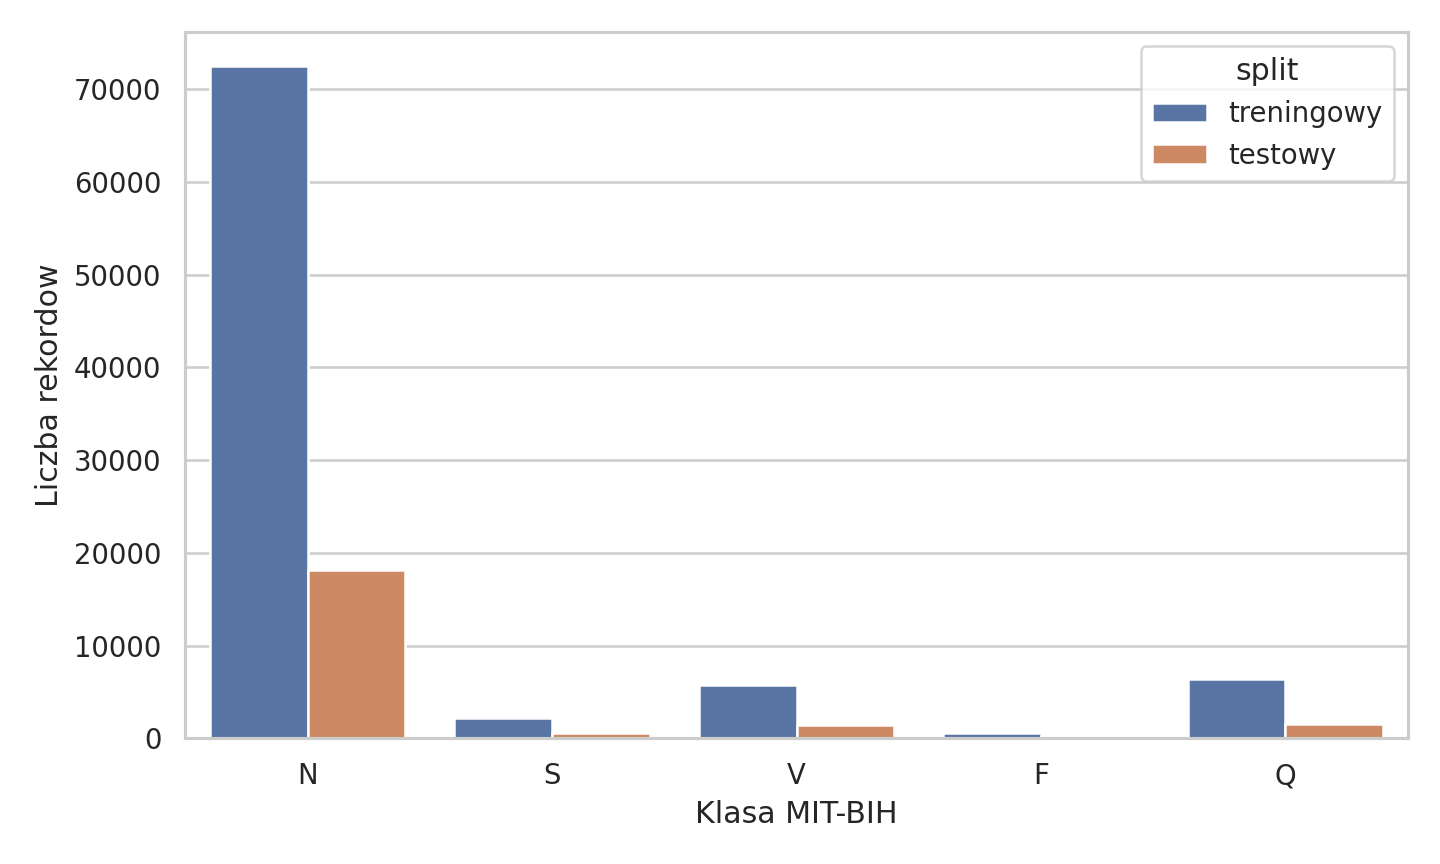
\includegraphics[width=0.86\textwidth]{class_distribution.png}
    \caption{Niezbalansowany rozkład klas w zbiorze treningowym i testowym.}
    \label{fig:class-distribution}
\end{figure}

\subsection{Preprocessing}
Wykonany preprocessing obejmował:
\begin{enumerate}
    \item wczytanie rekordów EKG ze zbioru treningowego i testowego,
    \item oddzielenie 187 kolumn sygnału od kolumny etykiety,
    \item sprowadzenie próbek do spójnej reprezentacji numerycznej,
    \item potraktowanie etykiet jako informacji pomocniczej do późniejszej analizy klas,
    \item wydzielenie części walidacyjnej ze zbioru treningowego,
    \item przygotowanie par uczących $(\mathbf{x}, \mathbf{x})$, ponieważ autoenkoder uczy się odtwarzać własne wejście.
\end{enumerate}

Sygnały w plikach Kaggle są już znormalizowane do przedziału $[0,1]$ i doprowadzone do stałej długości 187 próbek. W wielu rekordach końcowe próbki mają wartość zero, co oznacza dopełnienie krótszych segmentów. Z tego powodu przeprowadzono analizę przybliżonej długości niezerowej części sygnału. Wyniki przedstawiono w tabeli \ref{tab:padding-stats} oraz na rysunku \ref{fig:padding-lengths}.

\begin{table}[H]
    \centering
    \caption{Statystyki szacowanej długości niezerowej części sygnału.}
    \label{tab:padding-stats}
    \begin{tabular}{llllll}
\toprule
Zbior & Srednia & Odch. std. & Min & Mediana & Max \\
\midrule
treningowy & 111.69 & 27.46 & 17 & 109 & 187 \\
testowy & 111.42 & 27.44 & 10 & 108 & 187 \\
\bottomrule
\end{tabular}

\end{table}

\begin{figure}[H]
    \centering
    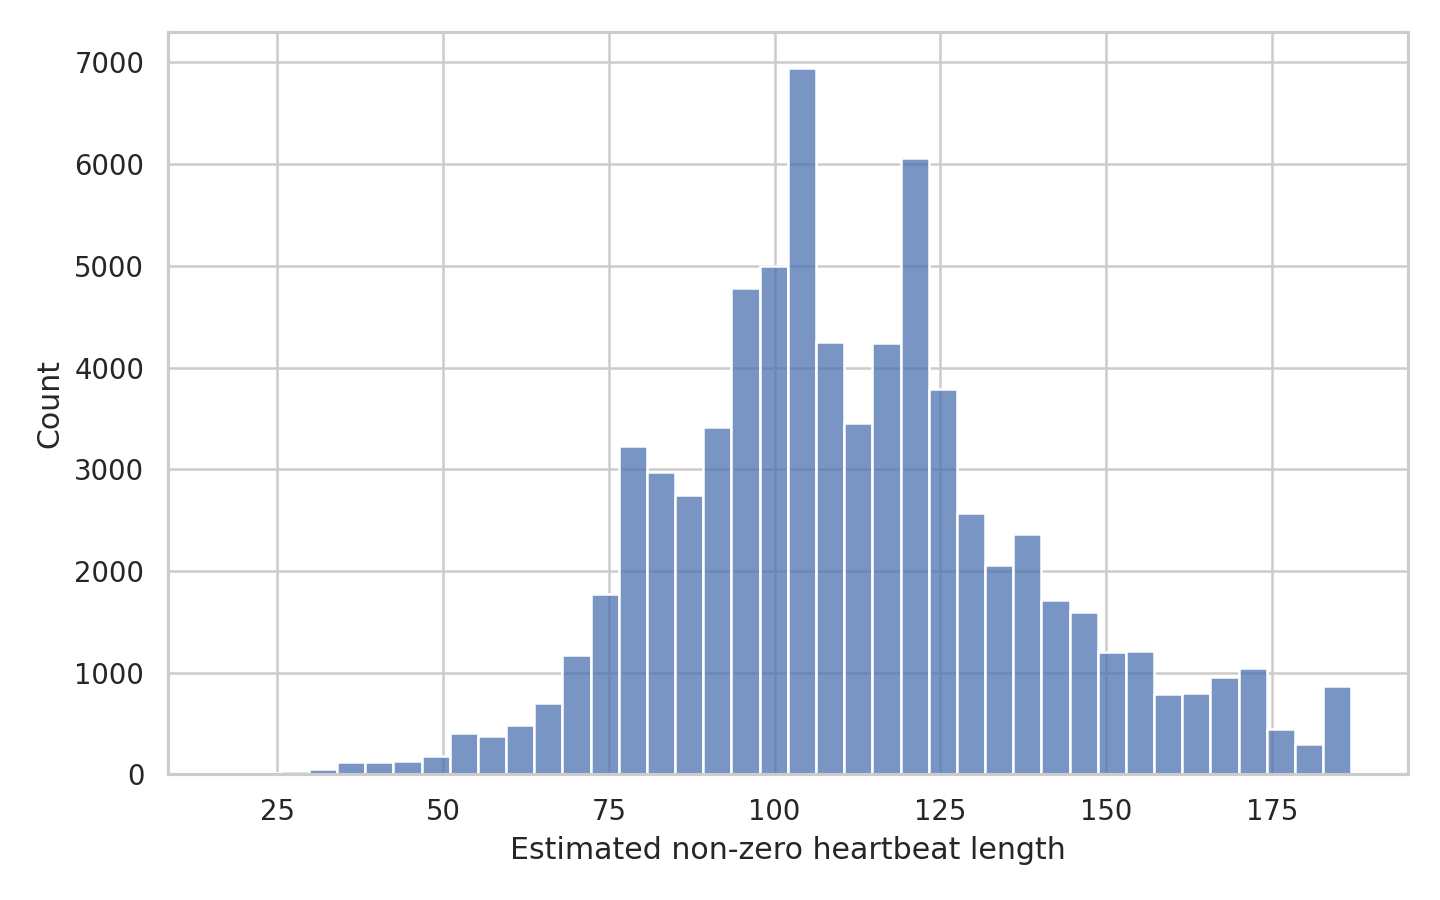
\includegraphics[width=0.86\textwidth]{padding_lengths.png}
    \caption{Histogram szacowanej długości sygnału przed końcowym zero-paddingiem.}
    \label{fig:padding-lengths}
\end{figure}

Dopełnienie zerami jest istotne dla kompresji, ponieważ model może nauczyć się bardzo dobrze odtwarzać końcowe fragmenty zawierające same zera. Dlatego w interpretacji wyników uwzględniono nie tylko MSE, ale także metryki względne, takie jak PRD i SNR.

\section{Autoenkoder MLP}
\subsection{Idea autoenkodera}
Autoenkoder jest siecią neuronową uczoną w trybie nienadzorowanym lub samonadzorowanym. Wejściem i celem uczenia jest ten sam obiekt. Model składa się z dwóch części:
\begin{itemize}
    \item enkodera $f_\theta$, który redukuje wymiar danych,
    \item dekodera $g_\phi$, który rekonstruuje dane wejściowe.
\end{itemize}
Jeżeli wymiar reprezentacji latentnej $K$ jest mniejszy od wymiaru wejścia, model musi nauczyć się zwartego opisu najważniejszych cech sygnału. Takie podejście jest klasycznym zastosowaniem autoenkoderów opisanym w literaturze uczenia głębokiego \cite{goodfellow2016}.

\subsection{Architektura}
Zastosowano autoenkoder typu MLP, czyli sieć w pełni połączoną. Dla każdego badanego wymiaru $K$ model miał tę samą część wejściową i wyjściową, a zmieniał się jedynie rozmiar warstwy latentnej. W eksperymencie właściwym użyto warstw:
\[
187 \rightarrow 2048 \rightarrow 1024 \rightarrow 512 \rightarrow 256 \rightarrow K
\]
w enkoderze oraz symetrycznego dekodera:
\[
K \rightarrow 256 \rightarrow 512 \rightarrow 1024 \rightarrow 2048 \rightarrow 187.
\]
W warstwach ukrytych zastosowano funkcję aktywacji ReLU. W warstwie wyjściowej użyto funkcji sigmoidalnej, ponieważ dane wejściowe są znormalizowane do zakresu $[0,1]$.

Z punktu widzenia kompresji najważniejsze jest to, że środkowa warstwa $K$ stanowi jedyną informację przekazywaną z enkodera do dekodera. W praktycznej interpretacji można ją traktować jako skompresowany opis uderzenia EKG. Jeżeli $K$ jest małe, model musi pominąć część szczegółów i zachować jedynie cechy najbardziej przydatne do rekonstrukcji. Jeżeli $K$ jest duże, w reprezentacji latentnej mieści się więcej informacji, ale maleje korzyść wynikająca z kompresji.

\subsection{Stopień kompresji}
Stopień kompresji zdefiniowano jako:
\[
    CR = \frac{187}{K}.
\]
Dla małych wartości $K$ otrzymuje się bardzo silną kompresję. Przykładowo dla $K=2$ reprezentacja ma tylko dwie liczby, więc formalny stopień kompresji wynosi $93{,}5$. Dla $K=96$ kompresja jest słabsza, ale model dysponuje znacznie większą przestrzenią do zapisania kształtu sygnału.

W eksperymentach sprawdzono wartości:
\[
K \in \{2, 4, 8, 16, 32, 64, 96\}.
\]

\section{Uczenie modelu}
\subsection{Funkcja celu}
Model uczono minimalizując średni błąd kwadratowy:
\[
    \mathcal{L}(\mathbf{x}, \hat{\mathbf{x}}) =
    \frac{1}{187}\sum_{i=1}^{187}(x_i-\hat{x}_i)^2.
\]
Jest to naturalna funkcja celu dla rekonstrukcji sygnału, ponieważ silnie karze większe odchylenia amplitudy.

\subsection{Parametry treningu}
Do uczenia wykorzystano:
\begin{itemize}
    \item optymalizator Adam,
    \item współczynnik uczenia $10^{-3}$,
    \item maksymalnie 80 epok,
    \item batch size 2048,
    \item podział walidacyjny 15\% ze zbioru treningowego,
    \item GPU CUDA oraz mixed precision AMP.
\end{itemize}

\begin{table}[H]
    \centering
    \caption{Podsumowanie przebiegu uczenia autoenkoderów MLP.}
    \label{tab:training}
    \begin{tabular}{lllll}
\toprule
$K$ & Epoki & Najl. MSE train & Najl. MSE val & Epoka \\
\midrule
2 & 80 & 0.004413 & 0.004443 & 70 \\
4 & 80 & 0.001773 & 0.001994 & 74 \\
8 & 80 & 0.001332 & 0.001440 & 77 \\
16 & 80 & 0.001638 & 0.001750 & 80 \\
32 & 80 & 0.001153 & 0.001272 & 80 \\
64 & 80 & 0.001266 & 0.001398 & 78 \\
96 & 80 & 0.001207 & 0.001292 & 80 \\
\bottomrule
\end{tabular}

\end{table}

\begin{figure}[H]
    \centering
    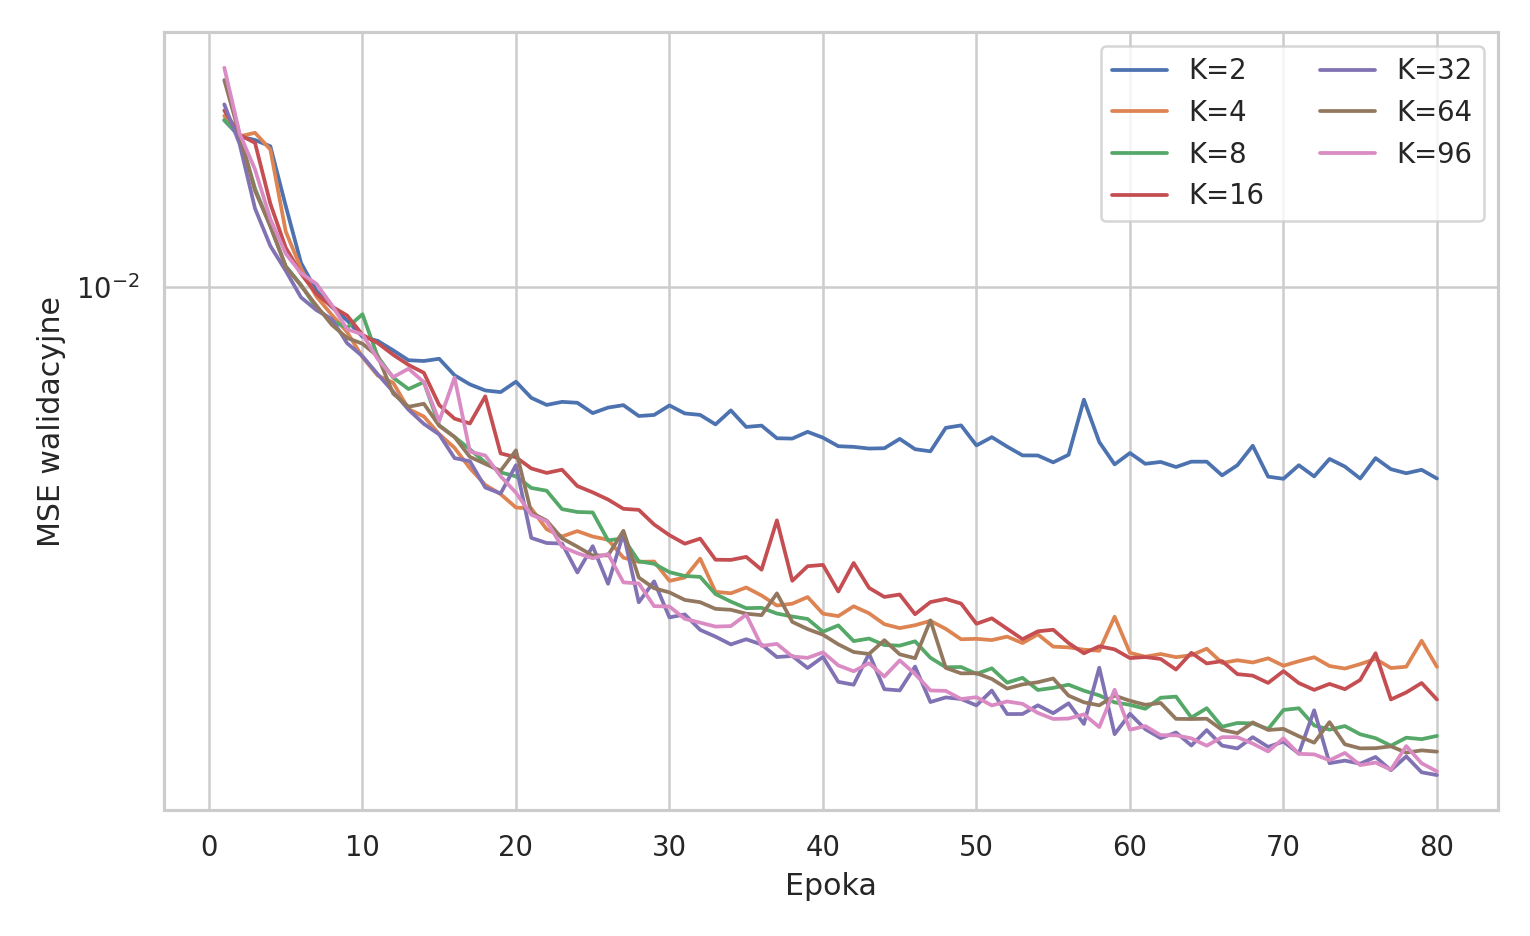
\includegraphics[width=0.9\textwidth]{validation_loss.png}
    \caption{Walidacyjny błąd MSE w kolejnych epokach dla różnych wartości $K$.}
    \label{fig:validation-loss}
\end{figure}

\section{Metryki jakości rekonstrukcji}
Do oceny jakości rekonstrukcji użyto kilku metryk, ponieważ pojedynczy wskaźnik nie opisuje w pełni zachowania modelu.

\subsection{RMSE i MAE}
RMSE określa pierwiastek ze średniego błędu kwadratowego:
\[
    RMSE = \sqrt{\frac{1}{N \cdot 187}\sum_{n=1}^{N}\sum_{i=1}^{187}
    (x_{n,i}-\hat{x}_{n,i})^2}.
\]
MAE mierzy średnią wartość bezwzględną błędu:
\[
    MAE = \frac{1}{N \cdot 187}\sum_{n=1}^{N}\sum_{i=1}^{187}
    |x_{n,i}-\hat{x}_{n,i}|.
\]

\subsection{PRD i PRDN}
PRD, czyli \textit{Percentage Root-mean-square Difference}, zdefiniowano jako:
\[
    PRD = 100 \cdot
    \sqrt{\frac{\sum(\mathbf{x}-\hat{\mathbf{x}})^2}
    {\sum \mathbf{x}^2+\varepsilon}}.
\]
PRDN jest wersją z centrowaniem sygnału:
\[
    PRDN = 100 \cdot
    \sqrt{\frac{\sum(\mathbf{x}-\hat{\mathbf{x}})^2}
    {\sum(\mathbf{x}-\bar{\mathbf{x}})^2+\varepsilon}}.
\]
Metryki PRD i PRDN są użyteczne w analizie sygnałów biomedycznych, ponieważ pokazują błąd względem energii sygnału.

\subsection{SNR i wskaźnik jakości}
Stosunek sygnału do szumu obliczono jako:
\[
    SNR = 10\log_{10}
    \frac{\sum \mathbf{x}^2+\varepsilon}
    {\sum(\mathbf{x}-\hat{\mathbf{x}})^2+\varepsilon}.
\]
Dodatkowo wprowadzono prosty wskaźnik jakości kompresji:
\[
    QS = \frac{CR}{PRD}.
\]
Wysoka wartość $QS$ oznacza korzystny kompromis: duży stopień kompresji przy względnie małym błędzie rekonstrukcji.

\section{Wyniki eksperymentów}
\subsection{Porównanie MLP i PCA}
Jako metodę odniesienia wykorzystano PCA. PCA dla danego $K$ znajduje najlepszą liniową podprzestrzeń minimalizującą błąd rekonstrukcji w sensie MSE. Autoenkoder MLP jest metodą nieliniową, ale nie ma gwarancji znalezienia globalnego optimum. Porównanie obu metod pozwala ocenić, czy nieliniowy model neuronowy uzasadnia swoją większą złożoność.

\begin{table}[H]
    \centering
    \caption{Metryki rekonstrukcji na zbiorze testowym.}
    \label{tab:metrics}
    \resizebox{\textwidth}{!}{\begin{tabular}{lllllllll}
\toprule
Metoda & $K$ & $CR$ & PRD & PRDN & SNR [dB] & RMSE & MAE & QS \\
\midrule
MLP autoencoder & 2 & 93.500 & 23.568 & 33.530 & 12.554 & 0.06706 & 0.03375 & 3.9673 \\
PCA & 2 & 93.500 & 43.952 & 62.531 & 7.140 & 0.12507 & 0.07194 & 2.1273 \\
MLP autoencoder & 4 & 46.750 & 15.867 & 22.574 & 15.990 & 0.04515 & 0.02147 & 2.9464 \\
PCA & 4 & 46.750 & 38.209 & 54.361 & 8.357 & 0.10872 & 0.05920 & 1.2235 \\
MLP autoencoder & 8 & 23.375 & 13.497 & 19.203 & 17.395 & 0.03841 & 0.01818 & 1.7319 \\
PCA & 8 & 23.375 & 32.652 & 46.454 & 9.722 & 0.09291 & 0.05051 & 0.7159 \\
MLP autoencoder & 16 & 11.688 & 14.790 & 21.042 & 16.601 & 0.04208 & 0.02003 & 0.7902 \\
PCA & 16 & 11.688 & 24.542 & 34.917 & 12.202 & 0.06983 & 0.03675 & 0.4762 \\
MLP autoencoder & 32 & 5.844 & 12.620 & 17.955 & 17.979 & 0.03591 & 0.01694 & 0.4631 \\
PCA & 32 & 5.844 & 15.406 & 21.918 & 16.246 & 0.04384 & 0.02150 & 0.3793 \\
MLP autoencoder & 64 & 2.922 & 13.237 & 18.833 & 17.564 & 0.03767 & 0.01775 & 0.2207 \\
PCA & 64 & 2.922 & 7.115 & 10.123 & 22.956 & 0.02025 & 0.00954 & 0.4107 \\
MLP autoencoder & 96 & 1.948 & 12.743 & 18.129 & 17.895 & 0.03626 & 0.01717 & 0.1529 \\
PCA & 96 & 1.948 & 4.123 & 5.866 & 27.696 & 0.01173 & 0.00526 & 0.4725 \\
\bottomrule
\end{tabular}
}
\end{table}

\begin{figure}[H]
    \centering
    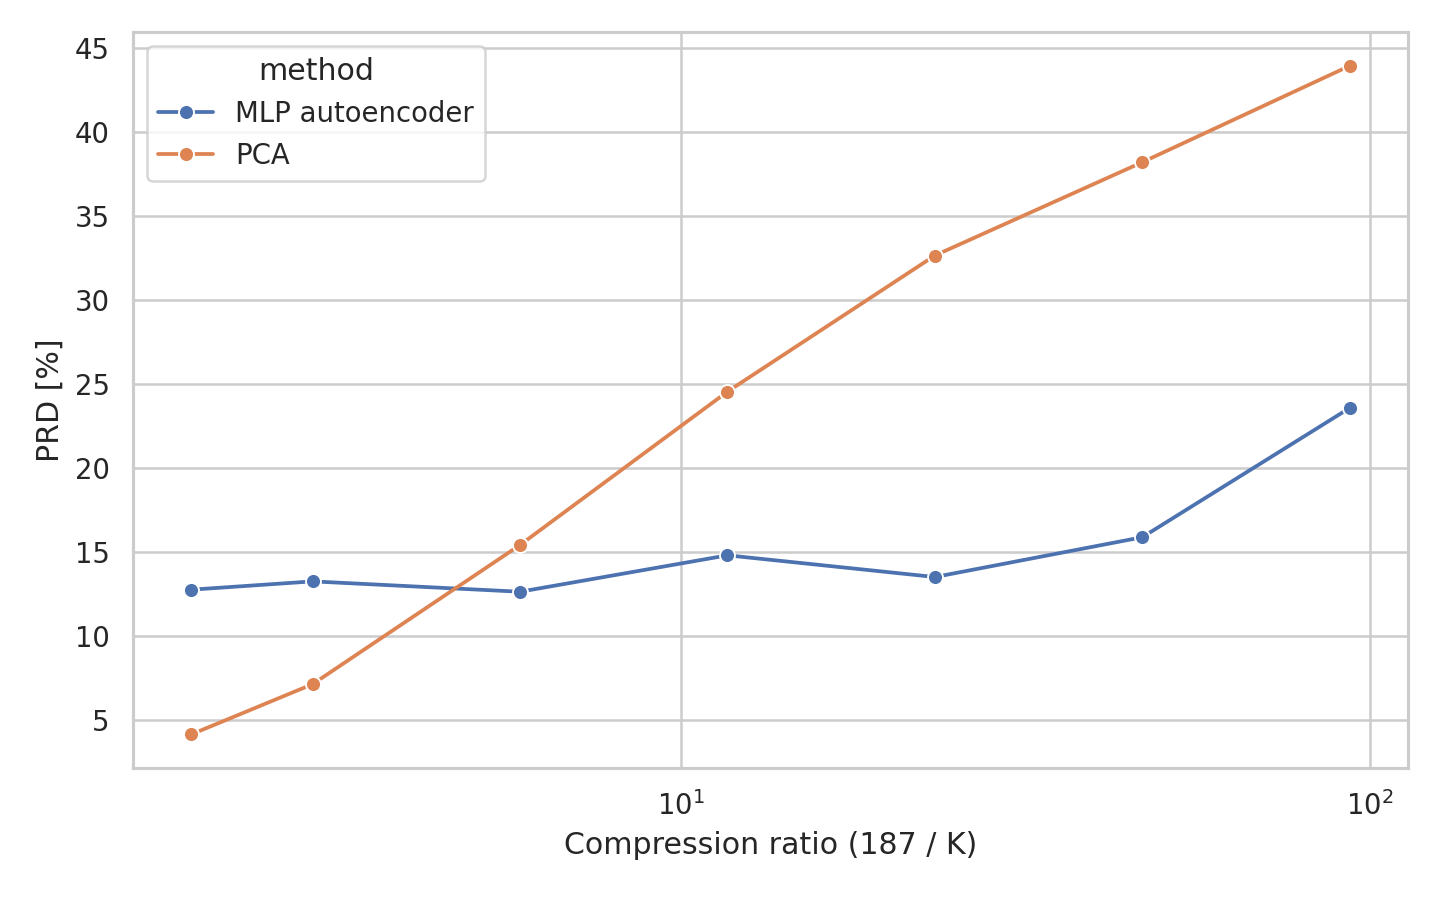
\includegraphics[width=0.86\textwidth]{cr_vs_prd.png}
    \caption{Zależność PRD od stopnia kompresji.}
    \label{fig:cr-prd}
\end{figure}

\begin{figure}[H]
    \centering
    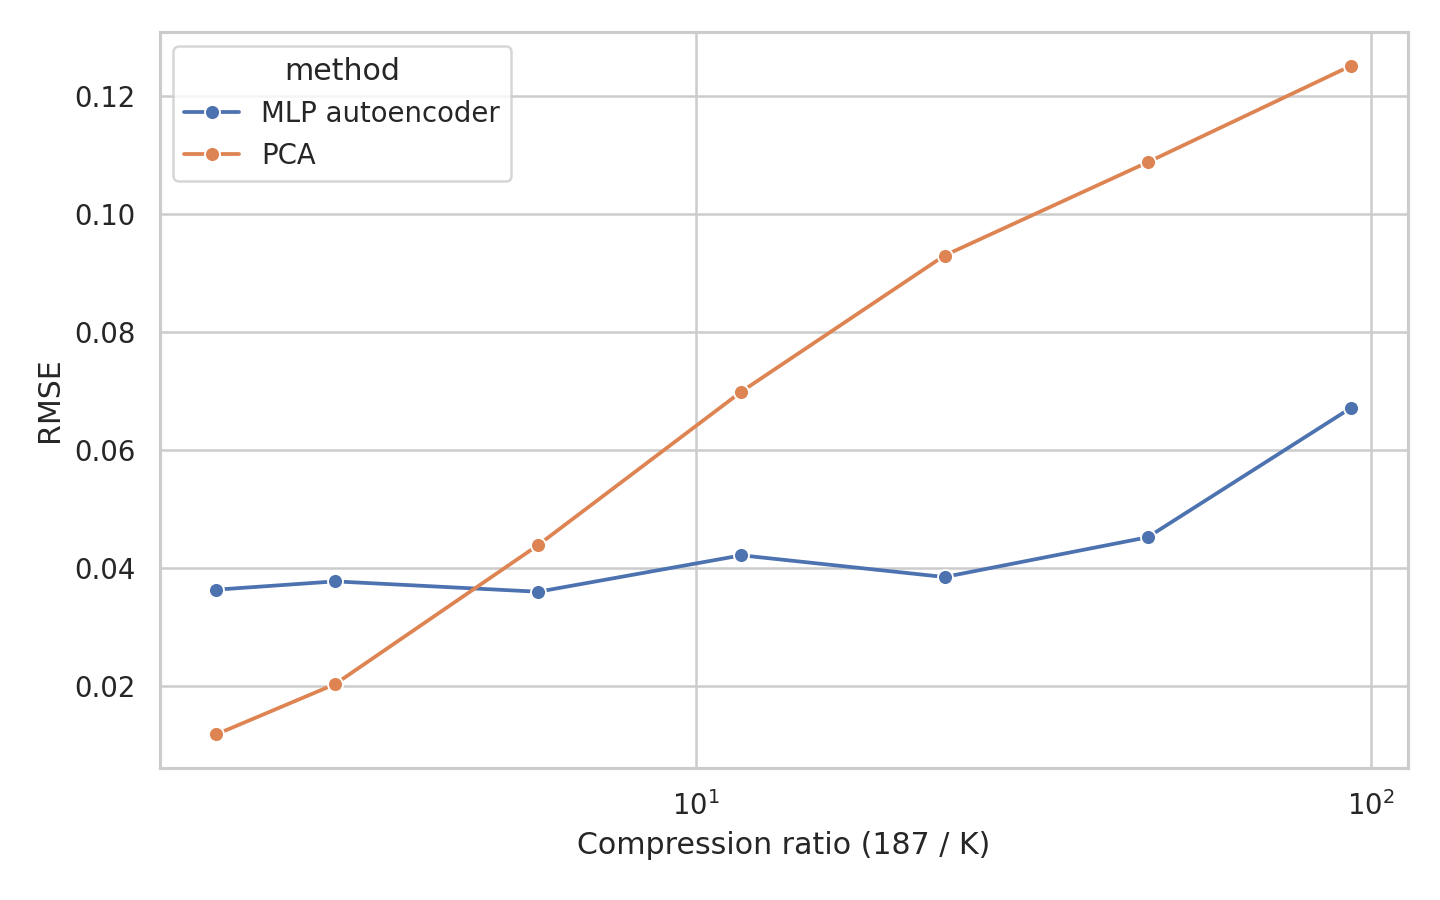
\includegraphics[width=0.86\textwidth]{cr_vs_rmse.png}
    \caption{Zależność RMSE od stopnia kompresji.}
    \label{fig:cr-rmse}
\end{figure}

\begin{figure}[H]
    \centering
    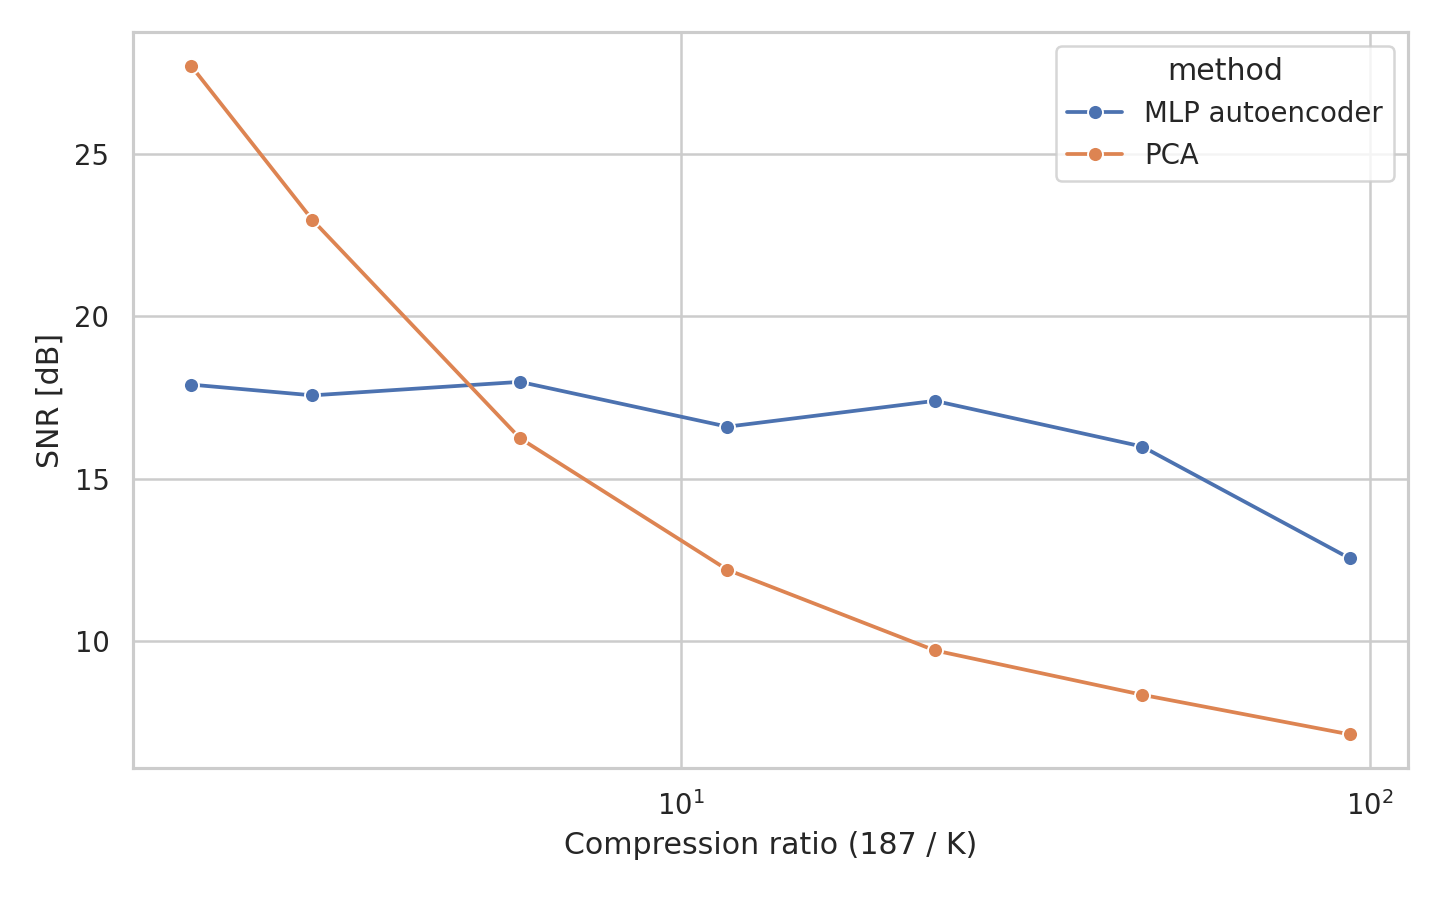
\includegraphics[width=0.86\textwidth]{cr_vs_snr.png}
    \caption{Zależność SNR od stopnia kompresji.}
    \label{fig:cr-snr}
\end{figure}

\begin{figure}[H]
    \centering
    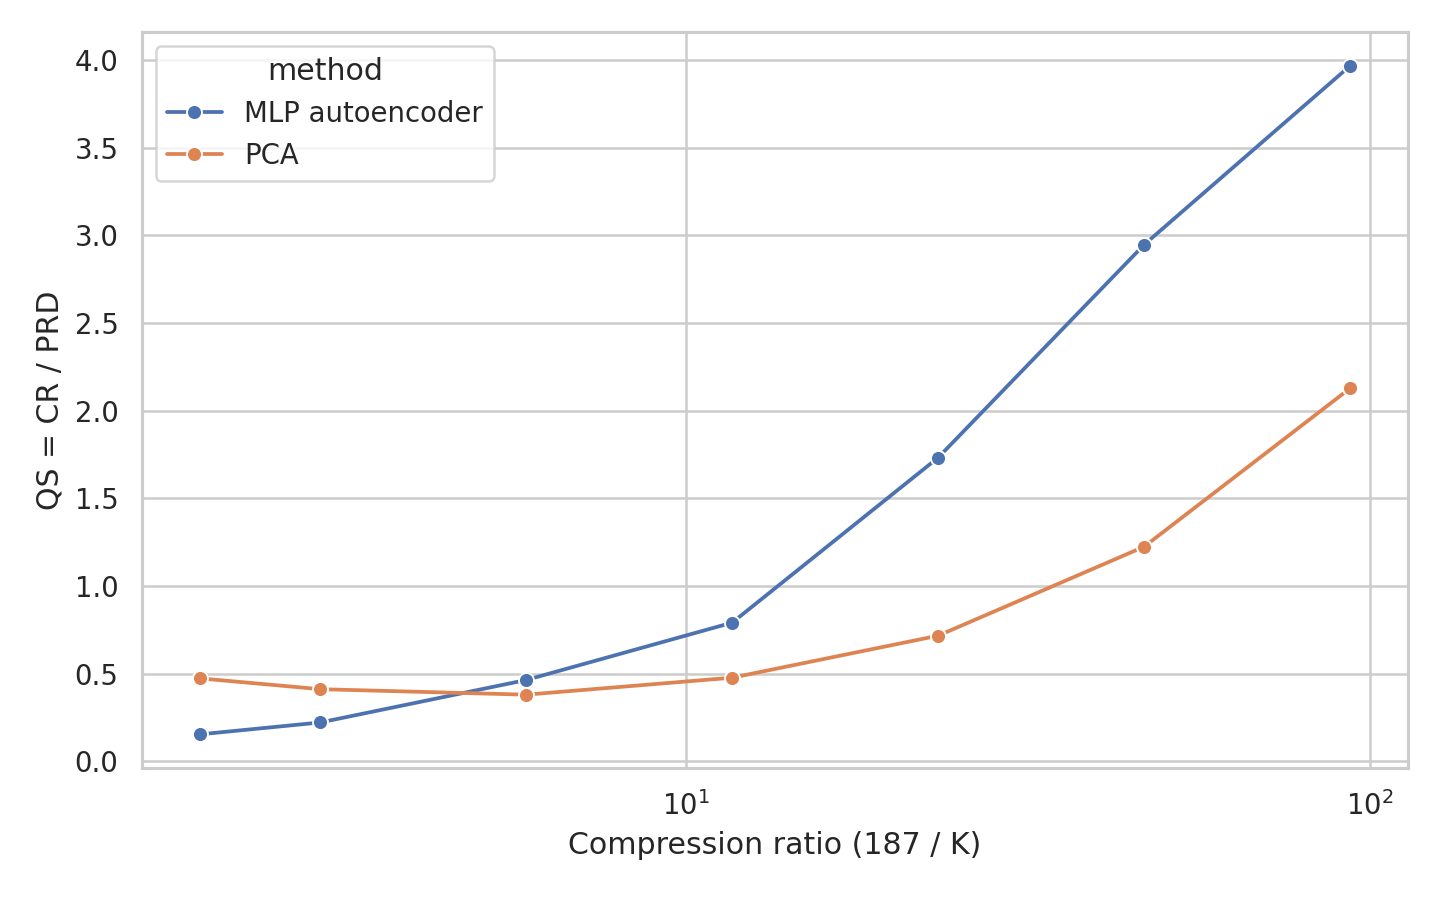
\includegraphics[width=0.86\textwidth]{cr_vs_qs.png}
    \caption{Zależność wskaźnika $QS=CR/PRD$ od stopnia kompresji.}
    \label{fig:cr-qs}
\end{figure}

Wyniki pokazują oczekiwany kompromis pomiędzy stopniem kompresji a jakością rekonstrukcji. Przy bardzo małym $K$ model musi zachować jedynie najbardziej dominujące cechy kształtu uderzenia. Wraz ze wzrostem $K$ rekonstrukcja staje się dokładniejsza, lecz maleje formalny stopień kompresji. Warto zauważyć, że najlepsza wartość samego PRD nie musi oznaczać najlepszego rozwiązania praktycznego, ponieważ model z dużym $K$ może poprawiać rekonstrukcję kosztem słabej kompresji.

Porównanie z PCA jest szczególnie istotne. PCA jest silną bazą odniesienia dla danych, których zmienność można dobrze opisać liniowo. Autoenkoder MLP może osiągać przewagę w wariantach o silniejszej kompresji, ponieważ nieliniowość pozwala lepiej odwzorować ograniczoną rozmaitość kształtów EKG. Dla większych wartości $K$ PCA może być konkurencyjne lub lepsze, co wynika z jej zamkniętej, stabilnej procedury optymalizacji liniowej. Oznacza to, że samo użycie sieci neuronowej nie gwarantuje automatycznie lepszej kompresji dla każdego poziomu $K$.

\subsection{Przykładowe rekonstrukcje}
Rysunki \ref{fig:recon-k8} i \ref{fig:recon-k16} przedstawiają przykładowe odtworzenia przebiegów. Na wykresach widać, że autoenkoder poprawnie zachowuje globalne położenie i główny kształt zespołu QRS, natomiast mniejsze elementy morfologii, takie jak drobne oscylacje lub szczegóły końcowej części sygnału, są wygładzane. Jest to typowe dla kompresji stratnej uczonej przez minimalizację MSE.

\begin{figure}[H]
    \centering
    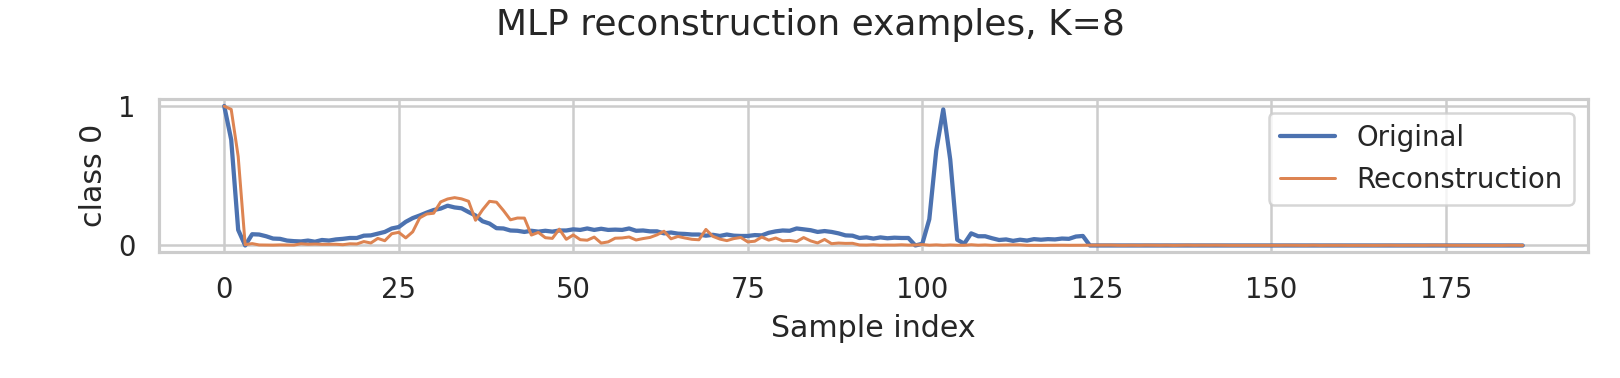
\includegraphics[width=0.92\textwidth]{reconstructions_k8.png}
    \caption{Przykładowe rekonstrukcje MLP dla $K=8$.}
    \label{fig:recon-k8}
\end{figure}

\begin{figure}[H]
    \centering
    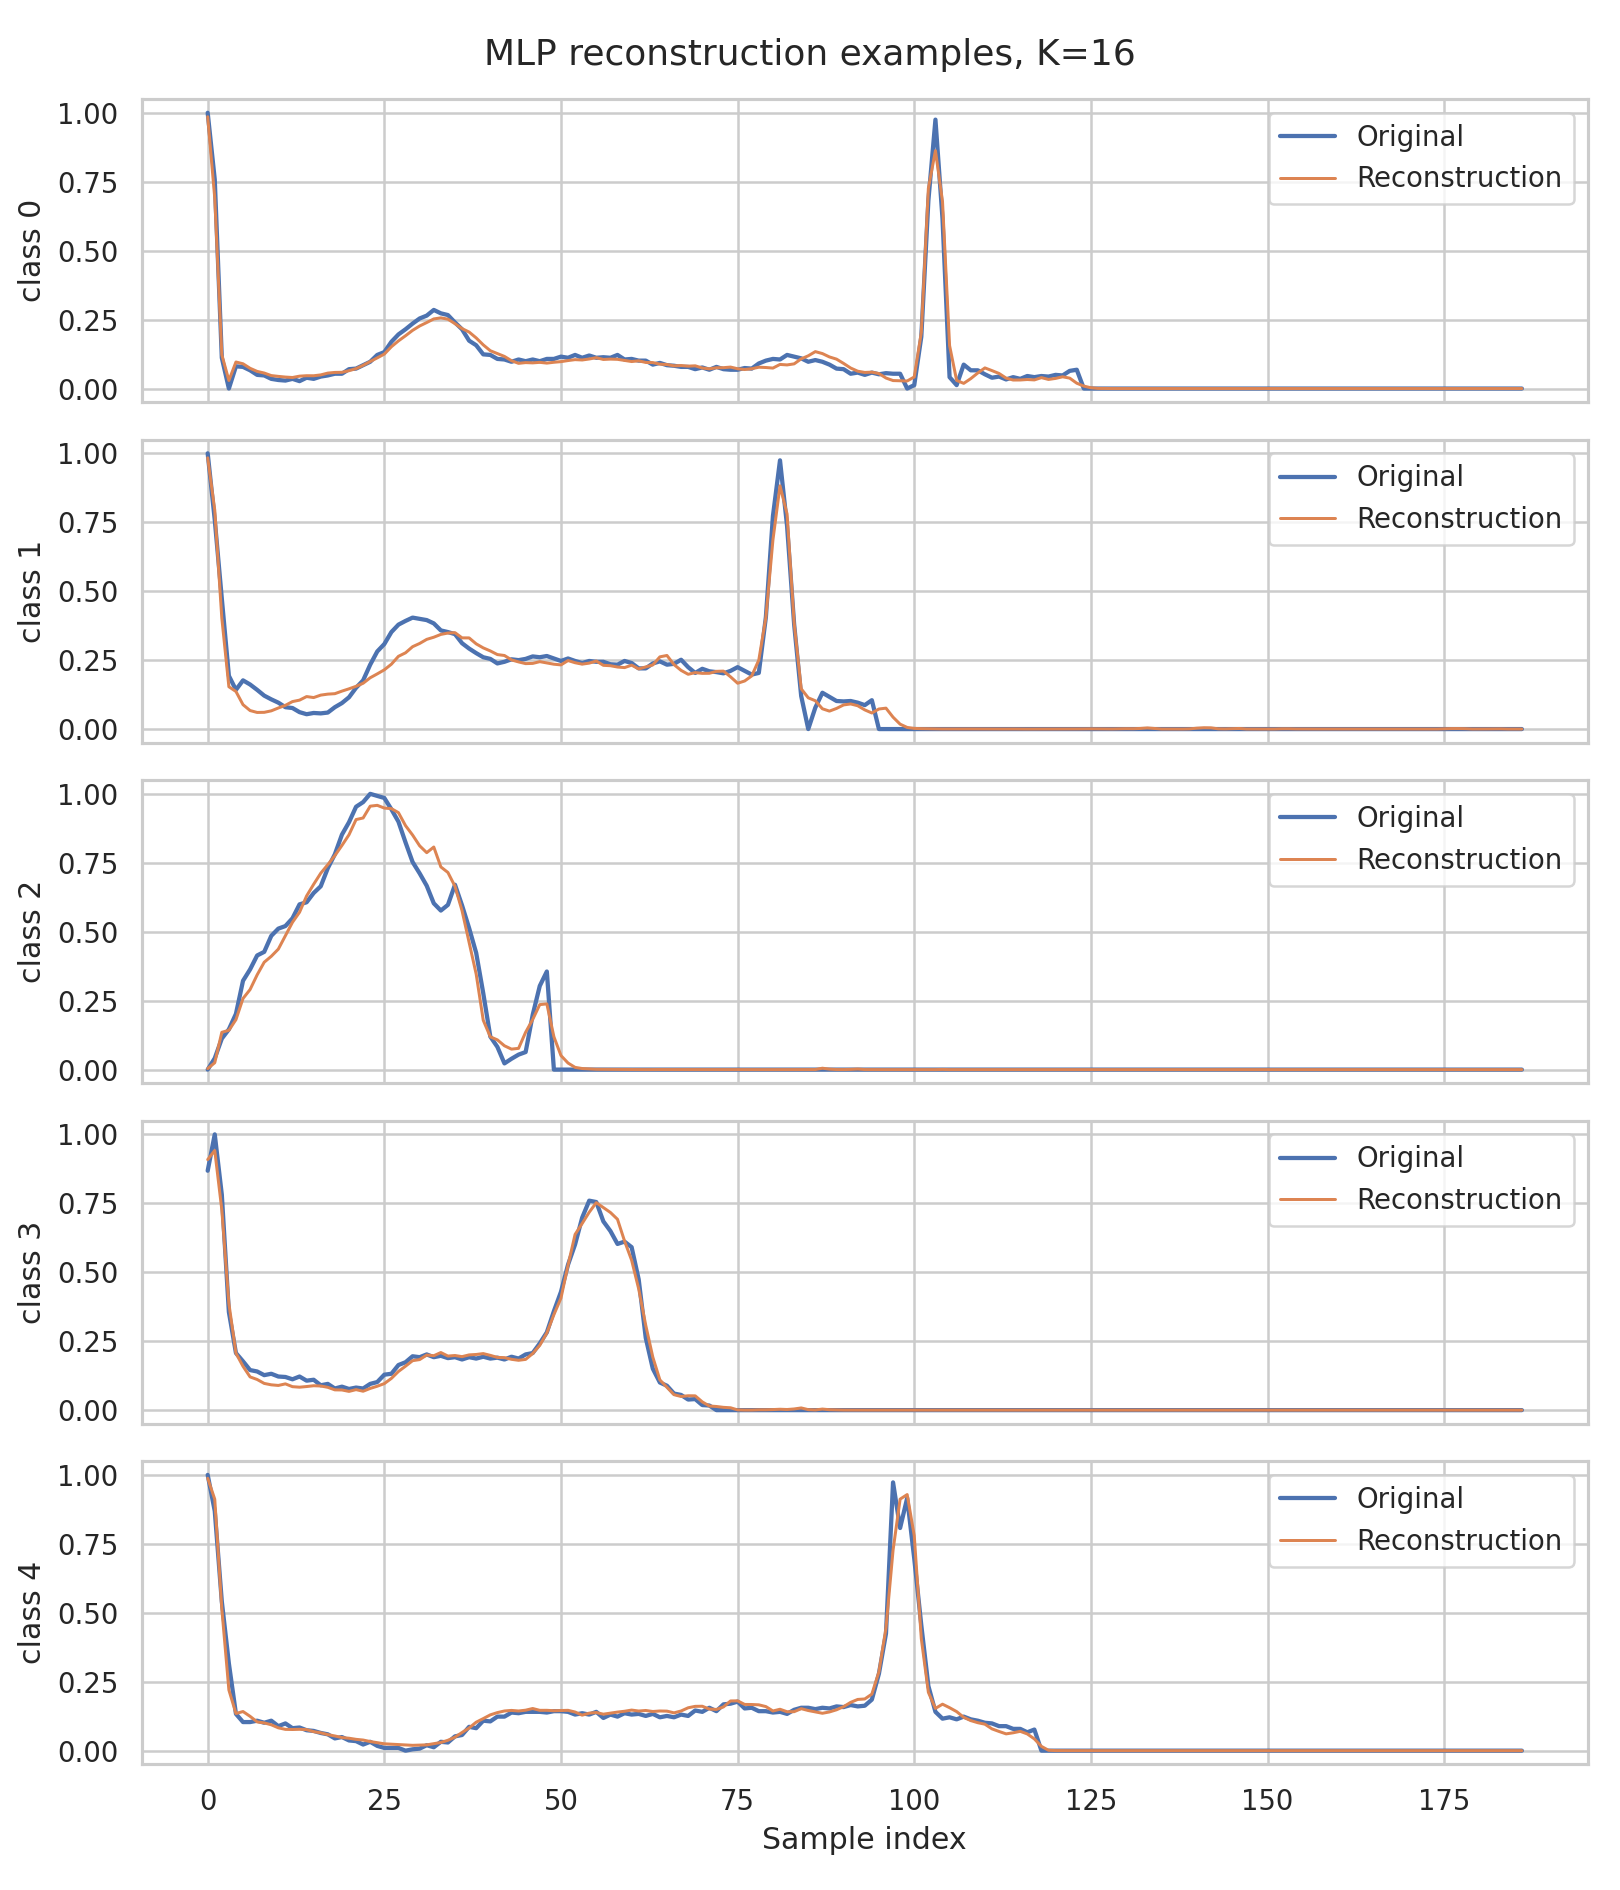
\includegraphics[width=0.92\textwidth]{reconstructions_k16.png}
    \caption{Przykładowe rekonstrukcje MLP dla $K=16$.}
    \label{fig:recon-k16}
\end{figure}

\subsection{Analiza klas}
Chociaż autoenkoder nie był uczony do klasyfikacji, etykiety klas pozwalają sprawdzić, czy jakość rekonstrukcji jest podobna dla różnych typów uderzeń. W zbiorze występuje silna nierównowaga klas: klasa normalna jest dominująca, a klasy rzadsze mają znacznie mniej przykładów. Taka struktura danych może powodować, że model lepiej odtwarza typowe kształty, a gorzej nietypowe lub rzadkie morfologie.

\begin{figure}[H]
    \centering
    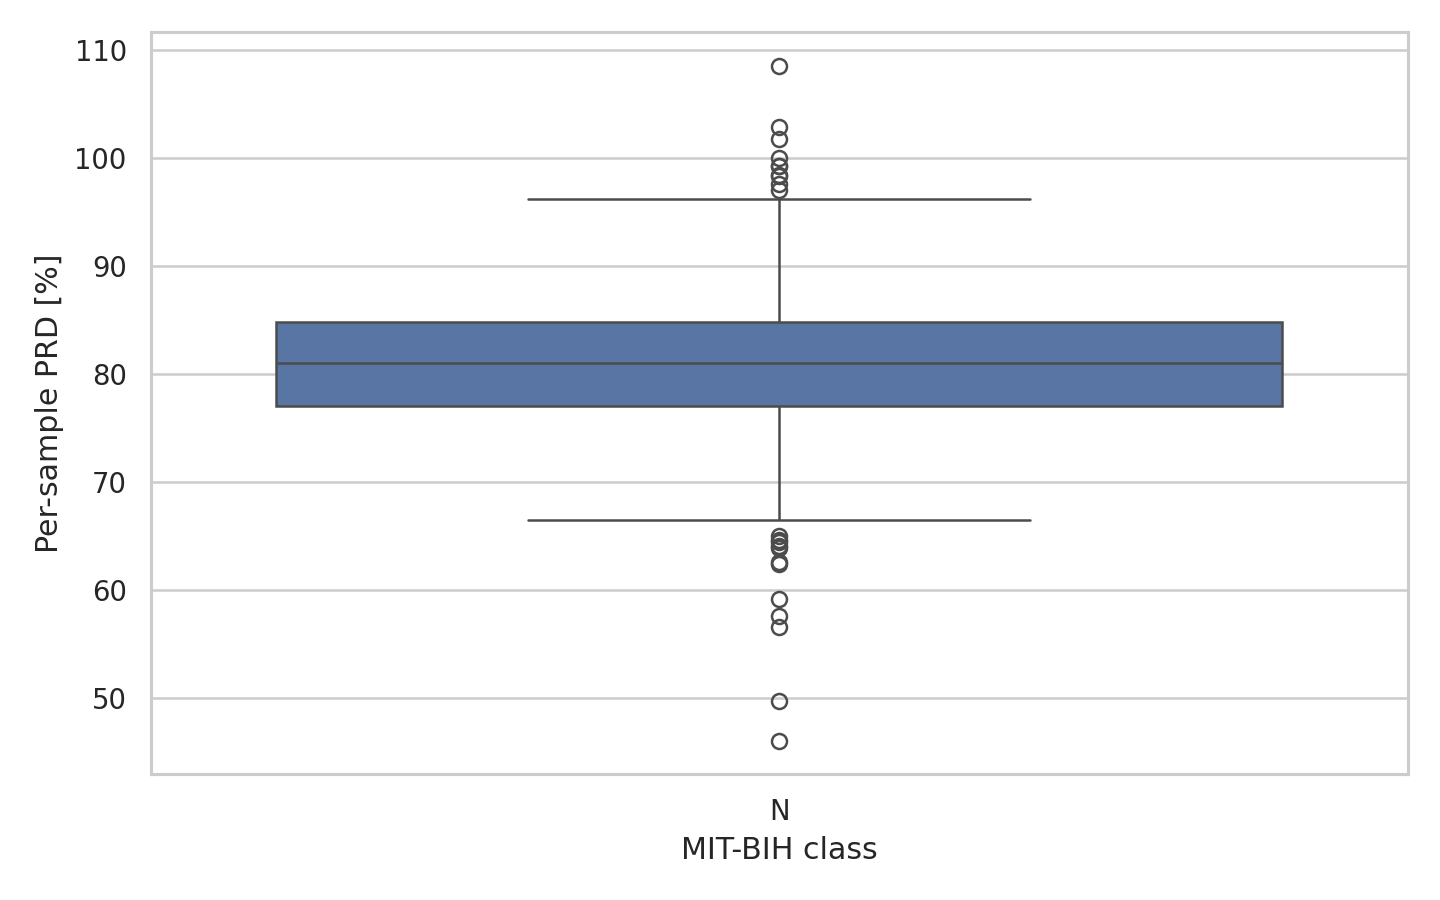
\includegraphics[width=0.86\textwidth]{prd_by_class_k8.png}
    \caption{Rozkład PRD dla poszczególnych klas MIT-BIH, $K=8$.}
    \label{fig:prd-class-k8}
\end{figure}

\begin{figure}[H]
    \centering
    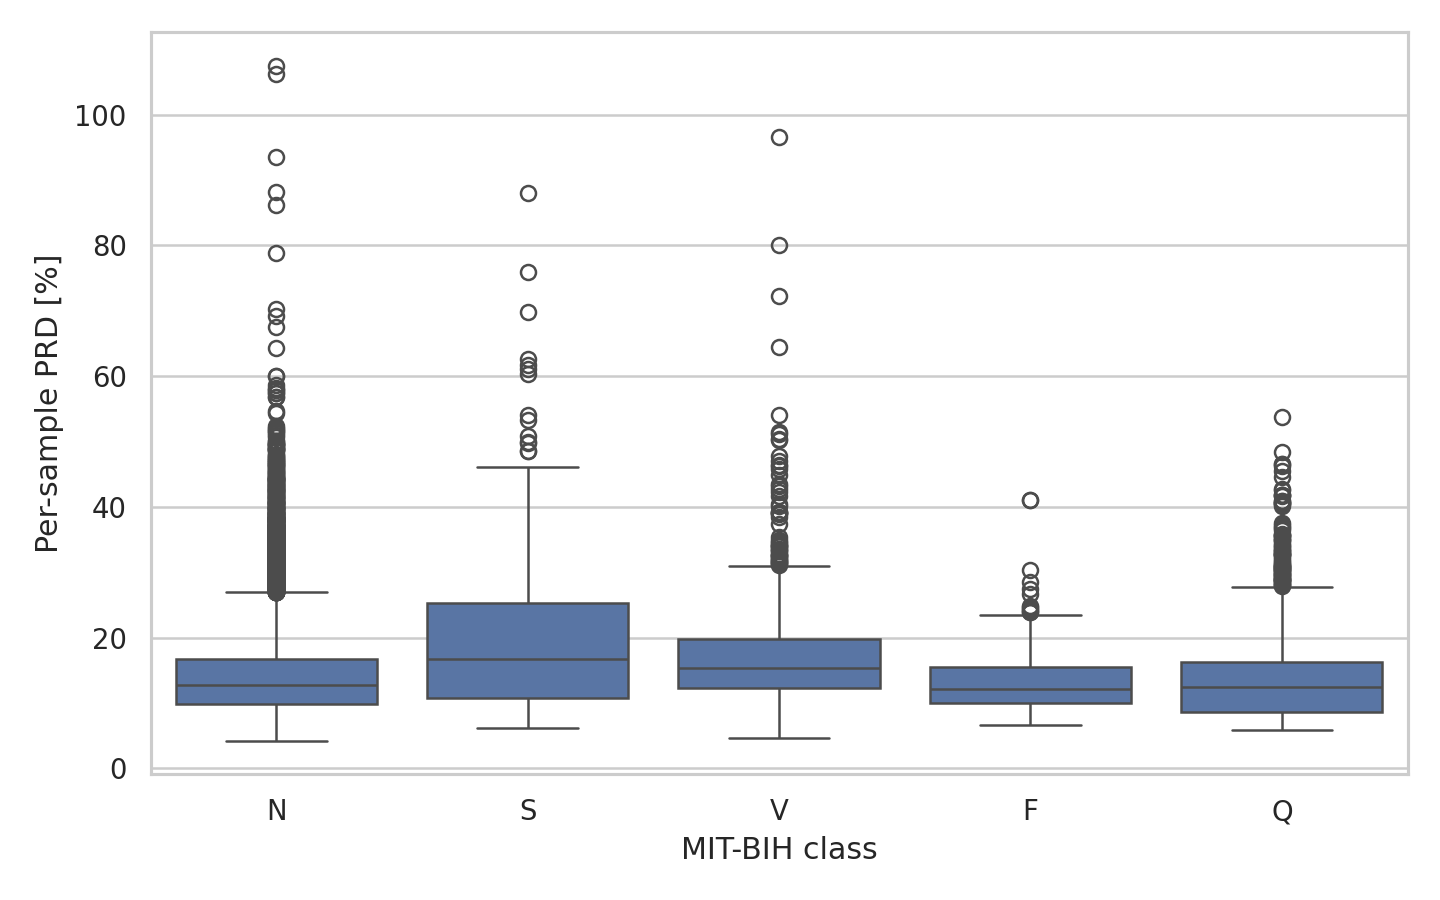
\includegraphics[width=0.86\textwidth]{prd_by_class_k16.png}
    \caption{Rozkład PRD dla poszczególnych klas MIT-BIH, $K=16$.}
    \label{fig:prd-class-k16}
\end{figure}

Analiza pudełkowa PRD pozwala stwierdzić, że błąd rekonstrukcji nie jest jednorodny pomiędzy klasami. Jest to zgodne z intuicją: autoenkoder optymalizuje średnią stratę na wszystkich rekordach, a więc klasy liczniejsze mają większy wpływ na gradient. W zastosowaniu medycznym należałoby rozważyć ważenie próbek, oversampling klas rzadkich albo osobne modele dla wybranych typów przebiegów.

\section{Procedura eksperymentalna}
Eksperyment zaplanowano tak, aby odpowiedzieć na dwa pytania: jak silnie można skompresować pojedyncze uderzenie EKG oraz jak szybko pogarsza się jakość rekonstrukcji przy zmniejszaniu wymiaru reprezentacji latentnej. Procedura składała się z następujących etapów:
\begin{itemize}
    \item przygotowanie danych i oddzielenie sygnałów od etykiet klas,
    \item wyznaczenie zbioru walidacyjnego służącego do obserwacji procesu uczenia,
    \item nauczenie osobnego autoenkodera dla każdej wartości $K$,
    \item rekonstrukcja wszystkich przykładów ze zbioru testowego,
    \item obliczenie metryk jakości rekonstrukcji,
    \item porównanie wyników MLP z metodą PCA przy tych samych wartościach $K$,
    \item analiza wykresów jakości, przykładów rekonstrukcji oraz rozkładów błędu w klasach.
\end{itemize}

Ważnym założeniem było zachowanie uczciwego porównania pomiędzy wariantami. Dla każdej wartości $K$ użyto tej samej architektury poza rozmiarem wąskiego gardła, tego samego podziału danych oraz tych samych metryk. Dzięki temu obserwowane różnice można interpretować głównie jako skutek zmiany stopnia kompresji, a nie jako efekt innej konfiguracji eksperymentu.

Wyniki analizowano na trzech poziomach. Pierwszy poziom stanowiły zagregowane miary błędu w tabeli metryk. Drugi poziom obejmował wykresy zależności $CR$ od PRD, RMSE, SNR i $QS$, które pokazują globalny kompromis między kompresją i jakością. Trzeci poziom polegał na wizualnej ocenie przykładowych rekonstrukcji oraz sprawdzeniu, czy błąd rozkłada się podobnie dla różnych klas MIT-BIH.

\section{Wnioski}
Zrealizowany projekt potwierdza, że autoenkoder MLP może zostać użyty jako stratny kompresor przebiegów EKG. Enkoder redukuje 187-próbkowy sygnał do wektora latentnego o wymiarze $K$, a dekoder odtwarza przebieg z tej reprezentacji. Najważniejszym parametrem sterującym kompromisem jest wymiar wąskiego gardła.

Dla małych wartości $K$ uzyskuje się bardzo wysoki stopień kompresji, ale rekonstrukcja traci część szczegółów. Dla większych wartości $K$ błąd maleje, lecz maleje też korzyść kompresji. W praktycznym zastosowaniu nie należy wybierać modelu wyłącznie na podstawie najniższego PRD; należy uwzględnić także $CR$, $QS$ oraz wymagania konkretnego systemu, np. transmisji danych z urządzenia przenośnego.

Porównanie z PCA pokazuje, że liniowa metoda odniesienia jest bardzo silna, zwłaszcza dla większych wymiarów reprezentacji. Autoenkoder MLP jest uzasadniony przede wszystkim wtedy, gdy zależy nam na nieliniowej kompresji i akceptujemy koszt treningu oraz strojenia hiperparametrów. Dalsze prace mogłyby obejmować autoenkodery konwolucyjne 1D, ważenie klas, inne funkcje straty oraz ocenę zachowania modelu na dłuższych, ciągłych fragmentach EKG.

\begin{thebibliography}{9}
\bibitem{kaggleheartbeat}
Shayan Fazeli, \textit{ECG Heartbeat Categorization Dataset}, Kaggle, \url{https://www.kaggle.com/datasets/shayanfazeli/heartbeat}.

\bibitem{kachuee2018}
M. Kachuee, S. Fazeli, M. Sarrafzadeh, \textit{ECG Heartbeat Classification: A Deep Transferable Representation}, arXiv:1805.00794, 2018.

\bibitem{moody2001}
G. B. Moody, R. G. Mark, \textit{The impact of the MIT-BIH Arrhythmia Database}, IEEE Engineering in Medicine and Biology Magazine, 20(3), 45--50, 2001.

\bibitem{goodfellow2016}
I. Goodfellow, Y. Bengio, A. Courville, \textit{Deep Learning}, MIT Press, 2016.
\end{thebibliography}

\end{document}
